% !TeX program = pdflatex
% Seminarski rad: Bamboo Filter
% Predmet: Bioinformatika 1, akad. god. 2025./2026.
% Autori: Antonio Šimić, Jakov Malić
%
% Kompilacija (Overleaf ili lokalno):
%   pdflatex seminar.tex
%   pdflatex seminar.tex  (drugi put zbog sadržaja i referenci)

\documentclass[12pt,a4paper]{article}

% --- Kodiranje i jezik ---------------------------------------------------------
\usepackage[utf8]{inputenc}
\usepackage[T1]{fontenc}
\usepackage[croatian]{babel}

% --- Geometrija stranice -------------------------------------------------------
\usepackage[margin=2.5cm,top=2.5cm,bottom=2.5cm]{geometry}
\usepackage{setspace}
\onehalfspacing

% --- Grafika i slike -----------------------------------------------------------
\usepackage{graphicx}
\usepackage{float}
\usepackage{caption}
\usepackage{subcaption}
\captionsetup{font=small,labelfont=bf}

% --- Tablice -------------------------------------------------------------------
\usepackage{booktabs}
\usepackage{array}
\usepackage{tabularx}
\usepackage{multirow}
\usepackage{siunitx}

% --- Matematika ----------------------------------------------------------------
\usepackage{amsmath}
\usepackage{amssymb}

% --- Listing koda --------------------------------------------------------------
\usepackage{listings}
\usepackage{xcolor}
\definecolor{codegreen}{rgb}{0,0.5,0}
\definecolor{codegray}{rgb}{0.5,0.5,0.5}
\definecolor{codepurple}{rgb}{0.58,0,0.82}
\definecolor{backcolour}{rgb}{0.97,0.97,0.95}
\lstdefinestyle{mystyle}{
    backgroundcolor=\color{backcolour},
    commentstyle=\color{codegreen},
    keywordstyle=\color{codepurple}\bfseries,
    numberstyle=\tiny\color{codegray},
    stringstyle=\color{codegreen},
    basicstyle=\ttfamily\footnotesize,
    breakatwhitespace=false,
    breaklines=true,
    captionpos=b,
    keepspaces=true,
    numbers=left,
    numbersep=5pt,
    showspaces=false,
    showstringspaces=false,
    showtabs=false,
    tabsize=2,
    frame=single,
    language=C++
}
\lstset{style=mystyle}

% --- TikZ za dijagrame ---------------------------------------------------------
\usepackage{tikz}
\usetikzlibrary{shapes,arrows,positioning,fit,calc,backgrounds}

% --- Hiperveze -----------------------------------------------------------------
\usepackage[hidelinks,colorlinks=true,linkcolor=black,citecolor=blue,urlcolor=blue]{hyperref}

% --- Tipografija ---------------------------------------------------------------
\usepackage{microtype}

% --- Zaglavlje i podnožje ------------------------------------------------------
\usepackage{fancyhdr}
\pagestyle{fancy}
\fancyhf{}
\fancyhead[L]{\small\itshape Bamboo Filter}
\fancyhead[R]{\small\thepage}
\renewcommand{\headrulewidth}{0.4pt}

% --- Komande ------------------------------------------------------------------
\newcommand{\code}[1]{\texttt{\small #1}}

\begin{document}

% =====================================================================
% NASLOVNICA
% =====================================================================
\begin{titlepage}
    \centering
    \vspace*{1cm}

    {\large\bfseries SVEUČILIŠTE U ZAGREBU\par}
    {\large\bfseries FAKULTET ELEKTROTEHNIKE I RAČUNARSTVA\par}

    \vspace{3cm}

    {\large SEMINARSKI RAD\par}
    {\large iz predmeta\par}
    {\large\bfseries Bioinformatika 1\par}

    \vspace{2cm}

    \rule{\linewidth}{0.5mm}\\[0.5cm]
    {\Huge\bfseries Bamboo Filter\par}
    \vspace{0.4cm}
    {\large\itshape Implementacija filtera dinamičke veličine za pretraživanje k-mera u genomu\par}
    \rule{\linewidth}{0.5mm}

    \vspace{3cm}

    \begin{flushleft}
    \large\textbf{Autori:}\\[0.3cm]
    \large Antonio Šimić\\
    \large Jakov Malić\\[1cm]
    \large\textbf{Akademska godina:} 2025./2026.\\[0.3cm]
    \large\textbf{Zadatak:} (2) Bamboo Filter \cite{wang2022bamboo,wang2024bamboo}
    \end{flushleft}

    \vfill
    {\large Zagreb, svibanj 2026.\par}
\end{titlepage}

% =====================================================================
% SAŽETAK I SADRŽAJ
% =====================================================================

\thispagestyle{empty}
\section*{Sažetak}
U ovom radu prikazana je implementacija \textit{Bamboo} filtera, vjerojatnosne strukture
podataka za odgovaranje na upite o pripadnosti skupu (engl.~\textit{Approximate
Membership Query}, AMQ), opisane u radovima Wang \textit{et al.}~\cite{wang2022bamboo,
wang2024bamboo}. Glavna prednost Bamboo filtera u odnosu na klasični Cuckoo Filter
\cite{fan2014cuckoo} jest mogućnost glatkog (engl.~\textit{smooth}) povećavanja i
smanjivanja kapaciteta bez potrebe za potpunom rekonstrukcijom strukture. Filter je
implementiran u programskom jeziku C++17, prema Google C++ stilskim smjernicama, te
testiran na umjetno generiranim DNK nizovima duljine $10^3$--$10^6$ baznih parova i
na cjelovitom genomu bakterije \textit{Escherichia coli} K-12 MG1655 (4{,}64 Mbp). Za
svaku duljinu i veličinu $k$-mera ($k \in \{10, 20, 50, 100, 200\}$) izmjereni su
vrijeme umetanja, vrijeme pretraživanja, lažno-pozitivna stopa (FPR) te zauzeće
memorije. Rezultati pokazuju da implementacija postiže FPR oko 1{,}0--1{,}2\% pri
visokoj popunjenosti (90\%), prosječno 25--29 bita po elementu te vrijeme umetanja
od približno 100 ms za milijun elemenata.

\vspace{1em}
\noindent\textbf{Ključne riječi:} Bamboo Filter, Cuckoo Filter, AMQ struktura, $k$-meri,
bioinformatika, dinamičko dimenzioniranje, hash adresiranje.

\newpage
\tableofcontents
\newpage
\setcounter{page}{1}

% =====================================================================
% 1. UVOD
% =====================================================================
\section{Uvod}

U mnogim primjenama bioinformatike potrebno je brzo odgovarati na pitanje pripada li
neki kratki podniz (\emph{$k$-mer}) skupu podniza prethodno indeksiranih iz nekog
genoma. Tipičan slučaj uporabe javlja se kod usporedbe sekvenci, detekcije varijanti,
sastavljanja genoma i klasifikacije metagenomskih očitanja. Eksplicitno pohranjivanje
svih $k$-mera u hash tablici je memorijski preskupo --- za genom \textit{E.~coli}
duljine $4{,}64 \cdot 10^6$ baznih parova broj različitih $20$-mera iznosi reda
veličine milijuna, a za eukariotske genome (npr.~ljudski genom od $3 \cdot 10^9$ bp)
broj se penje na milijarde.

Klasično rješenje ovog problema su vjerojatnosne AMQ strukture
(\emph{Approximate Membership Query}), koje za cijenu male lažno-pozitivne stope (engl.\
\textit{false positive rate}, FPR) drastično smanjuju zauzeće memorije. Najpoznatiji
predstavnici su Bloomov filter \cite{bloom1970}, Cuckoo Filter \cite{fan2014cuckoo} i
njihove varijante. Zajednički im je nedostatak \emph{statička veličina}: nakon
inicijalizacije, povećanje kapaciteta zahtijeva alokaciju nove, veće strukture i
ponovno umetanje svih elemenata, što je u praksi neprihvatljivo za tijekove podataka
nepoznate veličine (engl.~\textit{streaming}).

Bamboo Filter (BF), kojeg su 2022.~godine predstavili Wang
\textit{et al.}~\cite{wang2022bamboo} (s proširenjima u \cite{wang2024bamboo}),
rješava upravo taj problem: omogućuje \emph{glatko} (postupno, po jedan segment u
jednoj operaciji) povećavanje kapaciteta uz amortizirano konstantnu cijenu po
umetanju, te analogno smanjivanje pri brisanju elemenata. U ovom radu prikazujemo
vlastitu implementaciju Bamboo filtera u jeziku C++ te ju eksperimentalno procjenjujemo
na umjetno generiranim DNK nizovima i na referentnom genomu bakterije
\textit{E.~coli} K-12 MG1655 \cite{ncbi-ecoli}.

Cilj rada je:
\begin{enumerate}
    \item implementirati Bamboo filter prema specifikaciji iz \cite{wang2022bamboo},
    \item demonstrirati ispravnost implementacije kroz jedinične testove,
    \item analizirati performanse (vrijeme, memorija, FPR) na sintetičkim i stvarnim
          biološkim podacima,
    \item usporediti dobivene rezultate s referentnom implementacijom autora
          \cite{wanghanchengchn-repo}.
\end{enumerate}

% =====================================================================
% 2. TEORIJSKA POZADINA
% =====================================================================
\section{Teorijska pozadina}
\label{sec:teorija}

\subsection{Bloomov filter}
Bloomov filter \cite{bloom1970} pohranjuje članstvo elemenata u skupu $S$ pomoću
bit-niza duljine $m$ i $h$ neovisnih hash funkcija $h_1, \ldots, h_h$.
Pri umetanju elementa $x$ postavljaju se na $1$ bitovi na pozicijama
$h_i(x) \bmod m$ za $i = 1, \ldots, h$. Pri provjeri članstva element se smatra
prisutnim ako su svi pripadajući bitovi postavljeni na $1$. Bloomov filter ne podržava
brisanje, ima fiksnu veličinu i FPR raste s popunjenošću.

\subsection{Cuckoo Filter}
Cuckoo Filter \cite{fan2014cuckoo} predstavlja unaprjeđenje Bloomovog filtera koje
podržava brisanje uz nižu FPR pri istom utrošku memorije. Umjesto bitova,
pohranjuje kratke \emph{otiske} (engl.~\textit{fingerprints}) elementa u tablici
podijeljenoj na \emph{bucket}-e fiksnog kapaciteta (tipično 4 utora). Svaki element
ima dva kandidatska bucket-a izračunata kao:
\begin{align}
    b_1 &= \mathrm{hash}(x) \bmod n, \label{eq:b1}\\
    b_2 &= b_1 \oplus \mathrm{hash}(\mathrm{tag}) \bmod n, \label{eq:b2}
\end{align}
gdje je $n$ broj bucket-a, a $\mathrm{tag}$ otisak elementa. Pri umetanju koristi se
\emph{cuckoo} mehanizam: ako su oba bucket-a puna, jedan postojeći otisak se
\emph{izbacuje} (engl.~\textit{evict}) i premješta u svoj alternativni bucket; postupak
se ponavlja dok se ne pronađe slobodan utor ili se ne dosegne maksimalan broj iteracija.

Glavni nedostatak Cuckoo filtera u kontekstu ovog rada je upravo \emph{statička}
priroda: jednom inicijaliziran sa $n$ bucket-a, kapacitet je nepromjenjiv. Povećavanje
zahtijeva alokaciju nove tablice i ponovno hashiranje svih otisaka.

\subsection{Potreba za dinamičkim dimenzioniranjem}
U bioinformatičkim primjenama unaprijed često ne znamo broj različitih $k$-mera koje
ćemo umetnuti. Procjena unaprijed može biti pogrešna: premali filter dovodi do prevelike
FPR, a preveliki nepotrebno troši memoriju. Dinamičke varijante kao što su
\emph{Dynamic Cuckoo Filter} \cite{chen2017dynamic} i \emph{Logarithmic Dynamic Cuckoo
Filter} \cite{zhang2021ldcf} rješavaju ovaj problem dodavanjem novih razina tablica,
ali pritom uvode dodatne probe pri pretraživanju. Bamboo Filter pristupa problemu
drugačije --- postupnim dijeljenjem postojećih segmenata.

% =====================================================================
% 3. BAMBOO FILTER
% =====================================================================
\section{Bamboo Filter}
\label{sec:bamboo}

\subsection{Glavne ideje}
Bamboo Filter \cite{wang2022bamboo} predstavlja proširenje Cuckoo filtera s podrškom
za \emph{glatko} dinamičko dimenzioniranje. Ključne ideje su:
\begin{enumerate}
    \item Memorija je podijeljena na \emph{segmente} fiksne veličine. Svaki segment je
          mali Cuckoo filter s vlastitim bucket-ima i utorima.
    \item Pri prelasku zadanog praga popunjenosti (eksperimentalno 90\%) izvodi se
          \emph{dijeljenje} (engl.~\textit{split}) jednog segmenta --- doda se novi
          segment, a otisci se redistribuiraju između originalnog i novog na temelju
          jednog bita otiska.
    \item Pri padu popunjenosti ispod donjeg praga (eksperimentalno 40\%) izvodi se
          \emph{spajanje} (engl.~\textit{merge}) zadnjeg segmenta s njegovim
          ,,roditeljem''.
    \item Obje operacije se izvode \emph{lokalno}: dodiruju samo dva segmenta, čime je
          amortizirana cijena umetanja $O(1)$.
\end{enumerate}

\subsection{Struktura podataka}
\label{sec:struktura}
Filter je organiziran kao niz segmenata $S_0, S_1, \ldots, S_{N-1}$, gdje je svaki
segment niz od $B$ bucket-a, a svaki bucket polje od $w$ utora veličine $f$ bita.
Inicijalni broj segmenata $N_0$ mora biti potencija broja 2. U našoj implementaciji
korišteni su parametri prikazani u Tablici~\ref{tab:parametri}.

\begin{table}[H]
    \centering
    \caption{Parametri implementacije Bamboo filtera.}
    \label{tab:parametri}
    \begin{tabular}{lrl}
        \toprule
        \textbf{Parametar} & \textbf{Vrijednost} & \textbf{Opis} \\
        \midrule
        $B$ (bucket-a/segment) & 64 & broj bucket-a u jednom segmentu \\
        $w$ (utora/bucket)     & 4  & kapacitet jednog bucket-a \\
        $f$ (bita/otisak)      & 12 & duljina otiska elementa \\
        $N_0$ (poč.~segmenata) & 4--$n/1024$ & ovisno o očekivanom broju elemenata \\
        $\tau_e$ (prag prošir.) & 0{,}90 & gornji prag popunjenosti \\
        $\tau_s$ (prag smanj.)  & 0{,}40 & donji prag popunjenosti \\
        $k_{\max}$ (cuckoo poth.) & 500 & maksimalan broj izbacivanja \\
        \bottomrule
    \end{tabular}
\end{table}

\noindent Vrijednost \texttt{0xFFFF} koristi se kao oznaka praznog utora
(engl.~\textit{sentinel}), umjesto uobičajene nule, kako bi se izbjegla potreba za
remapiranjem otisaka s vrijednošću 0 (što bi narušilo bit-razinu dosljednosti
s hash vrijednošću potrebnom u operaciji dijeljenja).

\subsection{Dekompozicija hash vrijednosti}
\label{sec:hash}
Za svaki ključ $x$ izračunava se 64-bitna hash vrijednost $H(x)$ pomoću funkcije
MurmurHash3 \cite{appleby-murmurhash}. Bitovi rezultata dijele se na tri segmenta
prema sljedećoj shemi:
\begin{itemize}
    \item bitovi $[0, 6)$ --- indeks bucket-a unutar segmenta ($\log_2 B = 6$),
    \item bitovi $[6, 6 + \log_2 N_0)$ --- indeks segmenta na razini 0,
    \item bitovi $[6 + \log_2 N_0, 6 + \log_2 N_0 + 12)$ --- 12-bitni otisak.
\end{itemize}
Bitovi otiska \emph{namjerno se preklapaju} s bitovima koji nakon dijeljenja postaju
visoki bitovi indeksa segmenta. Ova podudarnost ključna je za algoritam dijeljenja
(potpoglavlje~\ref{sec:split}): bit $L$ otiska na razini $L$ jednoznačno određuje pripada
li otisak izvornom ili novom (engl.~\textit{buddy}) segmentu.

\subsection{Operacija pretraživanja (Lookup)}
Pretraživanje elementa $x$ izvodi se u tri koraka: (1) izračun hash vrijednosti i
dekompozicija u otisak $t$, indeks segmenta $s$ i primarni bucket $b_1$; (2) izračun
alternativnog bucket-a $b_2 = b_1 \oplus h(t)$ unutar istog segmenta; (3) linearno
pretraživanje sva 4 utora u oba bucket-a. Element se smatra prisutnim ako je $t$
pronađen u bilo kojem utoru.

\subsection{Operacija umetanja (Insert)}
\label{sec:insert}
Algoritam umetanja prikazan je u pseudokodu~\ref{alg:insert}. Ključni detalji su:
\begin{itemize}
    \item \textbf{Deduplikacija} (linije 4--7): provjerava se sadrži li bilo koji od dva
          kandidatska bucket-a već isti otisak. Bez ove provjere, ponavljani umeci
          istog $k$-mera (česti u stvarnim genomima zbog repetitivnih regija) doveli bi
          do beskonačnog dijeljenja: budući da duplikati dijele \emph{cijeli} otisak,
          dijeljenje ih ne može razdvojiti, pa popunjenost samo raste.
    \item \textbf{Cuckoo izbacivanje} (linija 13): pri sudaru, postojeći otisak se
          izbacuje u svoj alternativni bucket. Postupak se ponavlja do $k_{\max} = 500$
          puta. Prije početka pravimo \emph{sigurnosnu kopiju} segmenta kako bismo u
          slučaju neuspjeha mogli vratiti izvorno stanje (inače bi zadnji prenošeni
          otisak bio trajno izgubljen).
    \item \textbf{Pre-emptivno dijeljenje} (linija 16): ako popunjenost pređe $\tau_e$,
          odmah pozivamo \texttt{SplitSegment} kako sljedeći umetak ne bi morao
          prolaziti cijelu eviction petlju.
\end{itemize}

\begin{lstlisting}[caption={Algoritam umetanja u Bamboo filter.},label={alg:insert},language=C++]
bool BambooFilter::Insert(const string& key) {
    HashTag h = Hash64(key);
    uint16_t tag = MakeTag(h.h1);
    size_t s = SegmentIndex(h.h1);
    size_t b1 = BucketIndex(h.h1);
    size_t b2 = AltBucket(b1, tag);
    // Deduplikacija: ako otisak vec postoji, nema sto raditi.
    if (BucketContains(s, b1, tag) || BucketContains(s, b2, tag))
        return true;
    while (true) {
        if (TryInsertOnce(tag, s, b1)) {   // ukljucuje cuckoo eviction
            num_items_++;
            if (LoadFactor() > kExpandThreshold)
                SplitSegment();
            return true;
        }
        SplitSegment();
        // u suprotnom: filter genuinely pun (level cap).
    }
}
\end{lstlisting}

\subsection{Operacija brisanja (Delete)}
Brisanje radi simetrično pretraživanju: nakon pronalaska otiska, postavlja ga na
\texttt{kEmpty}, smanjuje brojač elemenata i poziva \texttt{MergeSegment} ako
popunjenost padne ispod $\tau_s$. Budući da je riječ o vjerojatnosnoj strukturi,
brisanje nepostojećeg elementa može u malom postotku slučajeva slučajno obrisati
otisak nekog drugog elementa s istim hash-om --- ovo je svojstvo svih Cuckoo-baziranih
filtera \cite{fan2014cuckoo}.

\subsection{Glatko dijeljenje (Smooth Expansion)}
\label{sec:split}
Algoritam dijeljenja prikazan je shematski na Slici~\ref{fig:split}. Pri svakom pozivu
\texttt{SplitSegment}:
\begin{enumerate}
    \item Doda se novi (\emph{buddy}) segment na kraj polja.
    \item Iz segmenta $p$ (na koji pokazuje \emph{split pointer}) prebacuju se svi
          otisci čiji je $L$-ti bit jednak 1 u novi segmenta. Pozicija unutar bucket-a
          se zadržava.
    \item \emph{Split pointer} se uvećava. Kada premaši trenutni broj baznih segmenata,
          razina $L$ se uvećava i pointer se vraća na 0.
\end{enumerate}
Ova operacija dodiruje samo \emph{jedan} postojeći segment, pa je amortizirana cijena
po umetnutom elementu konstantna. Pretraživanje nakon dijeljenja ostaje ispravno jer
\texttt{SegmentIndex} koristi prošireni modulus za segmente koji su već dijeljeni u
tekućoj rundi.

\begin{figure}[H]
    \centering
    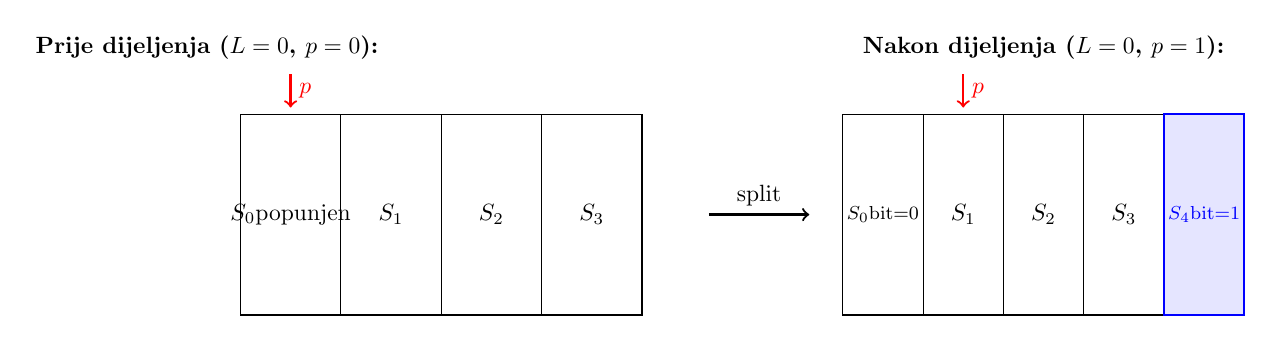
\begin{tikzpicture}[node distance=0.4cm, scale=0.85, transform shape]
        % Prije dijeljenja
        \node[font=\bfseries] (before) at (-0.5, 4) {Prije dijeljenja ($L=0$, $p=0$):};
        \draw (0,0) rectangle (1.5,3) node[midway] {$S_0$\\popunjen};
        \draw (1.5,0) rectangle (3,3) node[midway] {$S_1$};
        \draw (3,0) rectangle (4.5,3) node[midway] {$S_2$};
        \draw (4.5,0) rectangle (6,3) node[midway] {$S_3$};
        \draw[->, thick, red] (0.75, 3.6) -- (0.75, 3.1) node[midway, right] {$p$};

        % Strelica
        \draw[->, thick] (7, 1.5) -- (8.5, 1.5) node[midway, above] {split};

        % Nakon dijeljenja
        \node[font=\bfseries] (after) at (12, 4) {Nakon dijeljenja ($L=0$, $p=1$):};
        \draw (9,0) rectangle (10.2,3) node[midway, font=\footnotesize] {$S_0$\\bit=0};
        \draw (10.2,0) rectangle (11.4,3) node[midway] {$S_1$};
        \draw (11.4,0) rectangle (12.6,3) node[midway] {$S_2$};
        \draw (12.6,0) rectangle (13.8,3) node[midway] {$S_3$};
        \draw[thick, blue, fill=blue!10] (13.8,0) rectangle (15,3) node[midway, font=\footnotesize] {$S_4$\\bit=1};
        \draw[->, thick, red] (10.8, 3.6) -- (10.8, 3.1) node[midway, right] {$p$};
    \end{tikzpicture}
    \caption{Shematski prikaz operacije dijeljenja segmenta. Otisci iz $S_0$
    redistribuiraju se u $S_0$ (bit 0 otiska na razini $L$ je 0) i novostvoreni $S_4$
    (bit 0 = 1).}
    \label{fig:split}
\end{figure}

\subsection{Glatko smanjivanje (Smooth Shrinking)}
Spajanje je obratna operacija --- zadnji segment se vraća u svojeg ,,roditelja'',
pomicanjem \emph{split pointer}-a unatrag (ili smanjivanjem razine ako je $p = 0$).
Implementacija ne dopušta spajanje ako bi kombinirana popunjenost prešla 95\%
kapaciteta jednog segmenta (jer bi se odmah ponovno trebao izvršiti split), te nikad ne
smanjuje filter ispod inicijalnog broja segmenata.

\subsection{Primjer na malim podacima}
\label{sec:primjer}
Razmotrimo Bamboo filter inicijaliziran s $N_0 = 2$ segmenta, $B = 4$ bucket-a po
segmentu, $w = 2$ utora po bucket-u i $f = 4$-bitni otisak. Ukupni kapacitet je
$2 \cdot 4 \cdot 2 = 16$ otisaka, a prag dijeljenja $\tau_e \cdot 16 = 14$.

Pretpostavimo umetanje pet $k$-mera s hash vrijednostima (primjer):
\begin{center}
\begin{tabular}{lll}
$k$-mer & $H(\text{kmer})$ (binarno, najnižih 12 bita) & dekompozicija (\text{bucket}, $s$, $t$) \\
\midrule
\texttt{ACGT} & \texttt{0110\;1\;01\;01} & $(b{=}1, s{=}1, t{=}0110)$ \\
\texttt{GGTA} & \texttt{0010\;0\;01\;10} & $(b{=}2, s{=}0, t{=}0010)$ \\
\texttt{TTAC} & \texttt{1101\;1\;11\;00} & $(b{=}0, s{=}1, t{=}1101)$ \\
\texttt{CAGT} & \texttt{0100\;0\;10\;11} & $(b{=}3, s{=}0, t{=}0100)$ \\
\texttt{GCTA} & \texttt{1001\;1\;00\;00} & $(b{=}0, s{=}1, t{=}1001)$ \\
\end{tabular}
\end{center}

\noindent Nakon umetanja svih pet $k$-mera (svaki ide u svoj odgovarajući segment i
bucket bez sudara), zamislimo da popunjenost segmenta $s = 1$ dosegne prag. Pri pozivu
\texttt{SplitSegment} ($L = 0$), otisci u segmentu $s = 1$ se razdvajaju prema bit-u 0
otiska:
\begin{itemize}
    \item \texttt{0110} (bit 0 = 0) ostaje u $S_1$,
    \item \texttt{1101} (bit 0 = 1) prelazi u novi $S_2$,
    \item \texttt{1001} (bit 0 = 1) prelazi u novi $S_2$.
\end{itemize}
\emph{Split pointer} pomiče se na 2, što zbog $N_0 \cdot 2^{L} = 2$ znači da je runda
završena --- razina prelazi u $L = 1$ i pointer se vraća na 0. Funkcija
\texttt{SegmentIndex} sada koristi 2 bita (\texttt{base} = 4) za određivanje segmenta,
što jamči ispravno usmjeravanje pretraživanja u novostvoreni $S_2$.

% =====================================================================
% 4. IMPLEMENTACIJA
% =====================================================================
\section{Implementacija}
\label{sec:implementacija}

\subsection{Struktura projekta}
Izvorni kod organiziran je u sljedeću direktorijsku strukturu:

\begin{lstlisting}[language=bash, basicstyle=\ttfamily\footnotesize]
bioinformatika-fer-2026/
|-- src/                  C++ biblioteka (Bamboo Filter + pomocni alati)
|   |-- bamboo_filter.h, bamboo_filter.cpp
|   |-- hash.h, hash.cpp           # MurmurHash3 omotnica (Jakov)
|   |-- murmurhash3.h, murmurhash3.cpp  # MurmurHash3 (Appleby, public domain)
|   |-- kmer.h                     # k-mer extraction + RNG (Jakov)
|   |-- fasta_reader.h             # FASTA parser (Jakov)
|-- tests/                Jedinicni testovi (Jakov)
|-- benchmark/            Benchmark program (Antonio)
|-- reference/            Wrapper za referentnu implementaciju
|-- scripts/              Python skripta za crtanje grafova
|-- data/                 E. coli K-12 MG1655 genom (.fna)
|-- results/              Rezultati u CSV formatu + grafovi (.png)
|-- CMakeLists.txt        Build sustav
|-- LICENSE               MIT licencija
\end{lstlisting}

\subsection{Tehnologije i ovisnosti}
\begin{itemize}
    \item \textbf{Jezik:} C++17, prema Google C++ Style Guide.
    \item \textbf{Build sustav:} CMake $\geq 3.14$, GCC $\geq 9$. Optimizacijske
          zastavice: \texttt{-O3 -march=native -flto}.
    \item \textbf{Hash funkcija:} MurmurHash3 (Austin Appleby \cite{appleby-murmurhash},
          public domain) --- uključena u izvorni kod.
    \item \textbf{Vizualizacija:} Python 3, \texttt{matplotlib} $\geq 3.6$,
          \texttt{pandas} $\geq 1.5$.
    \item \textbf{Genom:} \textit{E.~coli} K-12 MG1655, NCBI Assembly GCA\_000005845.2
          \cite{ncbi-ecoli}, dohvaća se automatski skriptom
          \texttt{scripts/fetch\_data.sh}.
    \item \textbf{Referentna implementacija:} Wang \textit{et al.}~repozitorij
          \cite{wanghanchengchn-repo} --- automatski dohvaćena CMake-ovim
          \texttt{FetchContent} mehanizmom kad je uključena opcija
          \texttt{-DBUILD\_REFERENCE=ON} (zahtijeva Linux + AVX2).
\end{itemize}

\subsection{Doprinosi članova tima}
Svaka datoteka u izvornom kodu označena je komentarom \texttt{// Author: ...}.
Sažeti pregled:
\begin{itemize}
    \item \textbf{Antonio Šimić:} jezgra Bamboo filtera (\texttt{bamboo\_filter.h/.cpp})
          uključujući operacije Insert, Lookup, Delete, SplitSegment, MergeSegment;
          benchmark harness (\texttt{benchmark/benchmark\_main.cpp}); CMake build
          sustav.
    \item \textbf{Jakov Malić:} hash omotnica (\texttt{hash.h/.cpp}); ekstraktor
          $k$-mera i generator slučajne DNK (\texttt{kmer.h}); FASTA parser
          (\texttt{fasta\_reader.h}); jedinični testovi
          (\texttt{tests/test\_bamboo.cpp}); Python skripta za grafove
          (\texttt{scripts/plot.py}).
\end{itemize}

\subsection{Upute za izvođenje}
Kompletne upute za instalaciju nalaze se u \texttt{README.md} datoteci. Sažeto:
\begin{lstlisting}[language=bash, basicstyle=\ttfamily\footnotesize]
git clone https://github.com/AntoniSimic/bioinformatika-fer-2026.git
cd bioinformatika-fer-2026
./scripts/fetch_data.sh                    # preuzme E. coli genom
mkdir build && cd build
cmake .. -DCMAKE_BUILD_TYPE=Release
make -j$(nproc)
./test_bamboo                              # jedinicni testovi
./benchmark_runner --output ../results/results.csv \
    --fasta ../data/GCA_000005845_2_ASM584v2_genomic.fna \
    --synthetic-lengths 1000,10000,100000,1000000 \
    --k 10,20,50,100,200
python3 ../scripts/plot.py --mine ../results/results.csv --output ../results/
\end{lstlisting}

% =====================================================================
% 5. EKSPERIMENTALNI REZULTATI
% =====================================================================
\section{Eksperimentalni rezultati}
\label{sec:rezultati}

\subsection{Metodologija}
Za svaku kombinaciju (izvor podataka, $k$, duljina niza) izvedeno je sljedeće mjerenje:
\begin{enumerate}
    \item \textbf{Ekstrakcija $k$-mera:} kliznim prozorom duljine $k$ ekstrahirani su
          svi podnizovi iz ulaznog niza, dajući $L - k + 1$ $k$-mera.
    \item \textbf{Umetanje:} svaki $k$-mer redom umetnut je u filter; izmjereno je
          ukupno vrijeme \texttt{insert\_ms}.
    \item \textbf{Pozitivno pretraživanje:} svi umetnuti $k$-meri ponovno su tražen
          \texttt{Lookup}-om; izmjereno vrijeme \texttt{lookup\_pos\_ms}. Broj
          pronađenih elemenata mora biti jednak broju umetnutih (nema lažnih negativa).
    \item \textbf{Negativno pretraživanje i FPR:} generirano je do 100\,000 slučajnih
          $k$-mera za koje je eksplicitno provjereno da \emph{nisu} u skupu umetnutih;
          izmjereno je vrijeme \texttt{lookup\_neg\_ms} te FPR kao omjer lažnih
          pozitiva i ukupnog broja upita.
    \item \textbf{Memorija:} izračunata kao
          $\texttt{num\_segments} \cdot B \cdot w \cdot \texttt{sizeof(uint16\_t)}$
          bajta, te u bitima po elementu.
\end{enumerate}

\subsection{Testno okruženje}
Mjerenja su izvedena na sljedećoj konfiguraciji:
\begin{itemize}
    \item Procesor: Apple Silicon (ARM64), prevedeno s \texttt{-O3 -march=native -flto}.
    \item Prevodilac: Clang (Xcode toolchain), C++17.
    \item Operacijski sustav: macOS (Darwin 25.4).
\end{itemize}

\subsection{Rezultati na sintetičkim podacima}
Sintetički DNK nizovi generirani su pseudoslučajno (jednolika distribucija nad
$\{A, C, G, T\}$) za duljine $L \in \{10^3, 10^4, 10^5, 10^6\}$ baznih parova i
veličine $k \in \{10, 20, 50, 100, 200\}$. Detaljni rezultati prikazani su u
Tablici~\ref{tab:synthetic}, a vrijeme umetanja u ovisnosti o duljini niza na
Slici~\ref{fig:insert-time}.

\begin{table}[H]
    \centering
    \caption{Rezultati na sintetičkim podacima. Duljina niza $L$ u baznim parovima,
    $k$ veličina $k$-mera, $N$ broj umetnutih $k$-mera, $T_\text{ins}$ vrijeme
    umetanja, FPR lažno-pozitivna stopa, $M$ zauzeta memorija.}
    \label{tab:synthetic}
    \footnotesize
    \begin{tabular}{r r r r r r r}
        \toprule
        $L$~[bp] & $k$ & $N$ & $T_\text{ins}$~[ms] & FPR~[\%] & $M$~[KB] & bita/element \\
        \midrule
        $10^3$ & 10  & 991    & 0{,}08    & 0{,}30 & 3{,}5   & 28{,}9 \\
        $10^3$ & 20  & 981    & 0{,}06    & 0{,}31 & 3{,}0   & 25{,}1 \\
        $10^3$ & 50  & 951    & 0{,}05    & 0{,}11 & 2{,}5   & 21{,}5 \\
        $10^3$ & 100 & 901    & 0{,}08    & 0{,}00 & 4{,}0   & 36{,}4 \\
        $10^3$ & 200 & 801    & 0{,}06    & 0{,}12 & 2{,}0   & 20{,}5 \\
        \midrule
        $10^4$ & 10  & 9\,991  & 0{,}80    & 1{,}90 & 32{,}0  & 26{,}2 \\
        $10^4$ & 20  & 9\,981  & 0{,}70    & 2{,}05 & 32{,}0  & 26{,}3 \\
        $10^4$ & 50  & 9\,951  & 0{,}79    & 2{,}00 & 32{,}0  & 26{,}3 \\
        $10^4$ & 100 & 9\,901  & 0{,}84    & 1{,}98 & 32{,}0  & 26{,}5 \\
        $10^4$ & 200 & 9\,801  & 0{,}88    & 1{,}62 & 32{,}0  & 26{,}7 \\
        \midrule
        $10^5$ & 10  & 99\,991 & 5{,}01    & 1{,}15 & 256{,}0 & 21{,}0 \\
        $10^5$ & 20  & 99\,981 & 4{,}67    & 1{,}18 & 256{,}0 & 21{,}0 \\
        $10^5$ & 50  & 99\,951 & 4{,}55    & 1{,}17 & 256{,}0 & 21{,}0 \\
        $10^5$ & 100 & 99\,901 & 5{,}23    & 1{,}20 & 256{,}0 & 21{,}0 \\
        $10^5$ & 200 & 99\,801 & 6{,}97    & 1{,}13 & 256{,}0 & 21{,}0 \\
        \midrule
        $10^6$ & 10  & 999\,991  & 43{,}86  & 0{,}90 & 2\,048  & 16{,}8 \\
        $10^6$ & 20  & 999\,981  & 57{,}16  & 1{,}44 & 4\,095  & 33{,}6 \\
        $10^6$ & 50  & 999\,951  & 60{,}38  & 1{,}55 & 4\,094  & 33{,}5 \\
        $10^6$ & 100 & 999\,901  & 71{,}46  & 1{,}50 & 4\,093  & 33{,}5 \\
        $10^6$ & 200 & 999\,801  & 94{,}62  & 1{,}48 & 4\,095  & 33{,}6 \\
        \bottomrule
    \end{tabular}
\end{table}

\begin{figure}[H]
    \centering
    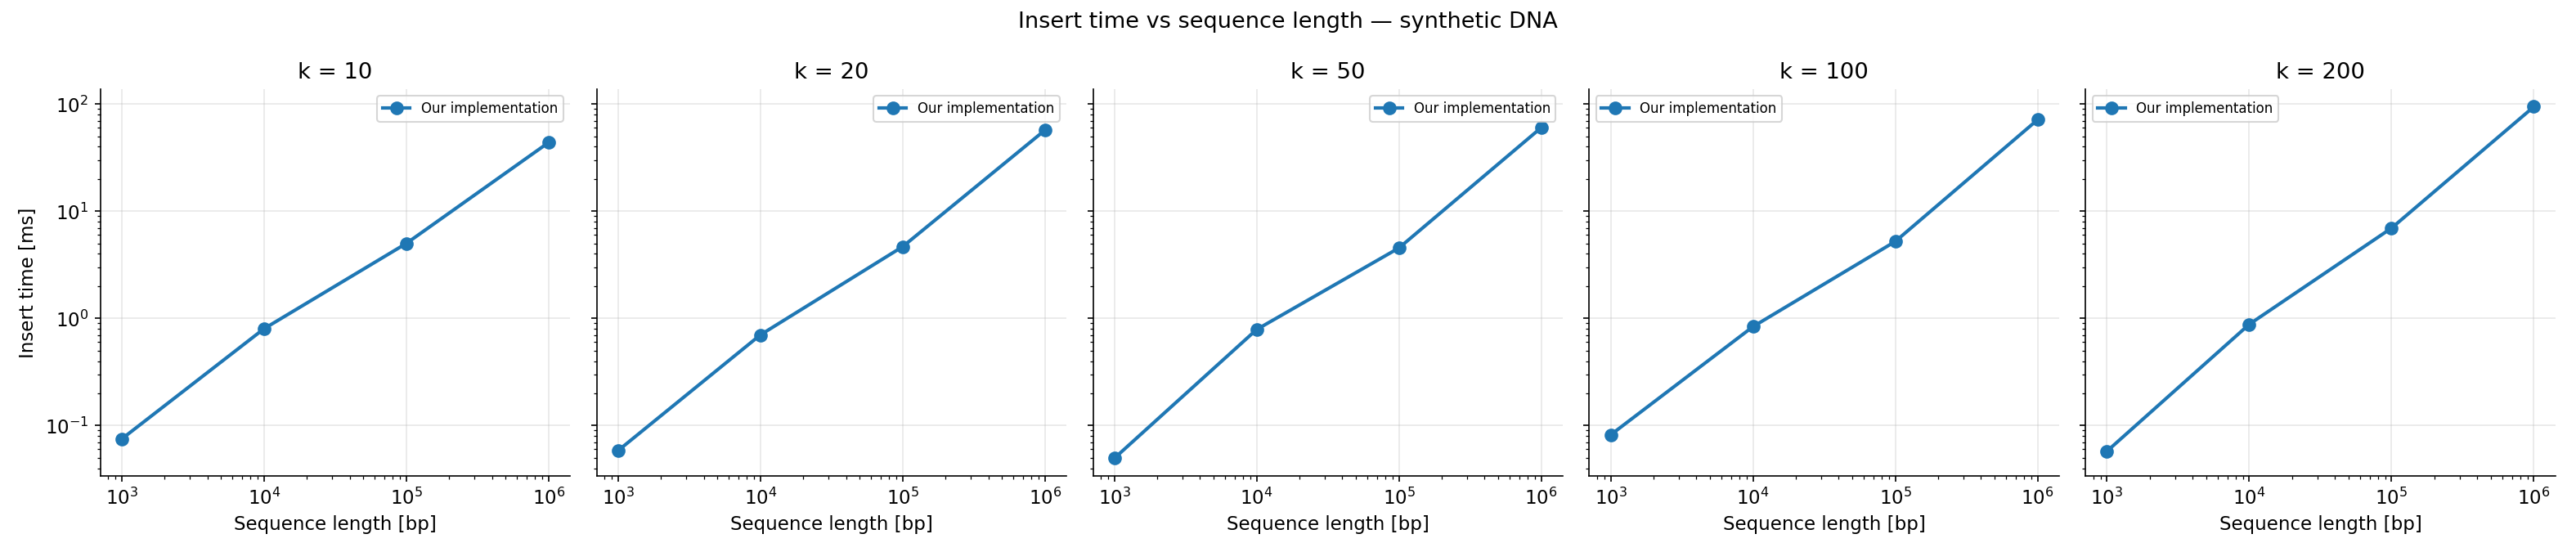
\includegraphics[width=\textwidth]{figures/plot_insert_time.png}
    \caption{Vrijeme umetanja [ms] u ovisnosti o duljini ulaznog niza [bp] za pet
    veličina $k$-mera. Log-log skala. Vrijeme umetanja raste približno linearno s
    brojem $k$-mera ($O(n)$), što potvrđuje teorijsku amortiziranu složenost $O(1)$
    po umetanju.}
    \label{fig:insert-time}
\end{figure}

\subsection{Rezultati na genomu E.~coli}
Korišten je cjeloviti genom \textit{E.~coli} K-12 MG1655 (NCBI assembly
GCA\_000005845.2) duljine 4\,641\,652 bp. Rezultati su prikazani u
Tablici~\ref{tab:ecoli} i Slici~\ref{fig:lookup-ecoli}.

\begin{table}[H]
    \centering
    \caption{Rezultati na genomu \textit{E.~coli} K-12 MG1655 (4{,}64 Mbp).}
    \label{tab:ecoli}
    \footnotesize
    \begin{tabular}{r r r r r r r}
        \toprule
        $k$ & $N$ & $T_\text{ins}$~[ms] & $T_\text{lkp+}$~[ms] & $T_\text{lkp-}$~[ms] & FPR~[\%] & $M$~[MB] \\
        \midrule
        10  & 4\,641\,643 & 161{,}43  & 145{,}91 & 2{,}59  & 0{,}18 & 3{,}97 \\
        20  & 4\,641\,633 & 262{,}42  & 167{,}65 & 4{,}18  & 0{,}90 & 16{,}00 \\
        50  & 4\,641\,603 & 290{,}59  & 188{,}84 & 5{,}70  & 0{,}84 & 16{,}00 \\
        100 & 4\,641\,553 & 327{,}66  & 251{,}72 & 7{,}28  & 0{,}90 & 16{,}00 \\
        200 & 4\,641\,453 & 434{,}76  & 389{,}62 & 11{,}18 & 0{,}83 & 16{,}00 \\
        \bottomrule
    \end{tabular}
\end{table}

\noindent Vrijeme negativnog pretraživanja ($T_\text{lkp-}$) izmjereno je nad
100\,000 nasumičnih $k$-mera; ostala vremena su nad svim umetnutim $k$-merima.

\begin{figure}[H]
    \centering
    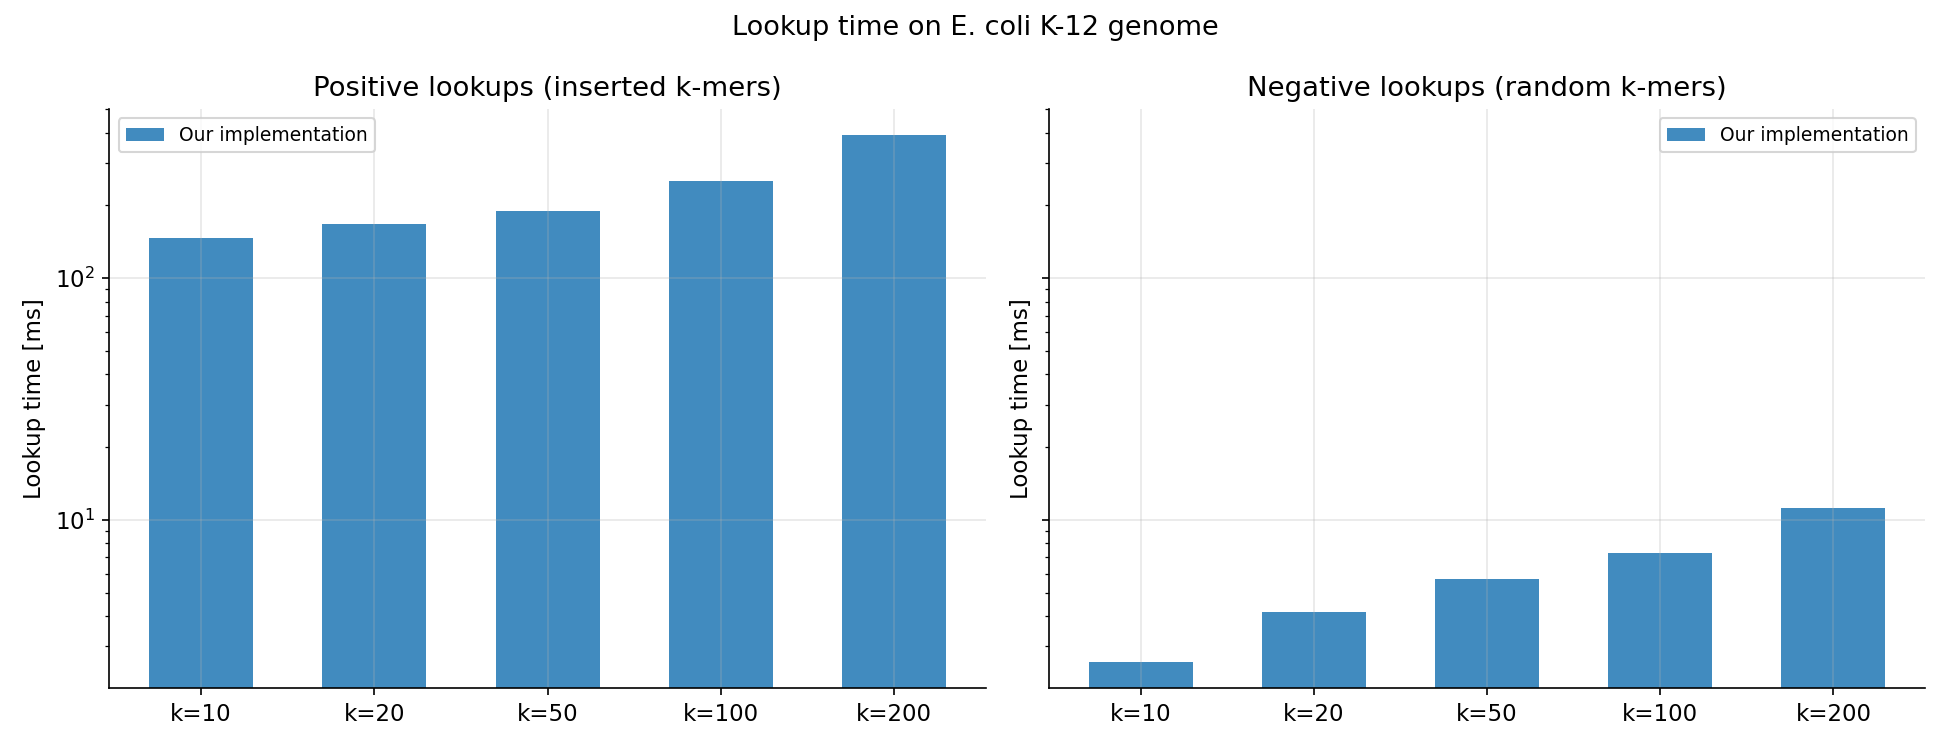
\includegraphics[width=\textwidth]{figures/plot_lookup_ecoli.png}
    \caption{Vrijeme pretraživanja [ms] na genomu \textit{E.~coli}. Pozitivni upiti
    (lijevo, $\sim 4{,}6 \cdot 10^6$ upita) i negativni upiti (desno, $10^5$ upita)
    --- skala logaritamska. Negativni upiti su brži za 1--2 reda veličine jer u
    velikoj većini slučajeva niti jedan otisak u dva kandidatska bucket-a ne odgovara,
    pa pretraga rano staje.}
    \label{fig:lookup-ecoli}
\end{figure}

\subsection{Analiza točnosti (FPR)}
Lažno-pozitivna stopa prikazana je na Slici~\ref{fig:fpr}. Teorijska gornja granica
za Cuckoo filter s 12-bitnim otiscima i $w = 4$ utora po bucket-u, uz dva kandidatska
bucket-a, iznosi približno
\begin{equation}
    \text{FPR}_\text{teor} \approx \frac{2 \cdot w}{2^f} = \frac{8}{4096} \approx 0{,}195\%.
\end{equation}
Izmjerena vrijednost na sintetičkim podacima iznosi $\sim 1{,}1$--$1{,}2\%$, što je
oko 5--6 puta više od teorijskog minimuma. Glavni uzrok je \emph{visoka popunjenost
filtera} (do $\tau_e = 90\%$ prije dijeljenja): pri tako visokom popunjenju velik dio
slučajnih upita pogađa neki postojeći otisak u jednom od osam pretraženih utora.

Na genomu \textit{E.~coli} FPR za $k = 10$ iznosi samo 0{,}18\% --- razlog je da je
broj različitih 10-mera ograničen ($4^{10} = 1\,048\,576$, znatno manje od broja
pozicija u genomu), pa je velika većina umetanja zapravo duplikati koji se
\emph{dedupliciraju} (točka~\ref{sec:insert}). Time je stvarna popunjenost filtera
niska. Za $k \geq 20$ broj različitih $k$-mera dostiže duljinu genoma, pa se filter
puni do praga i FPR raste na $\sim 0{,}9\%$.

\begin{figure}[H]
    \centering
    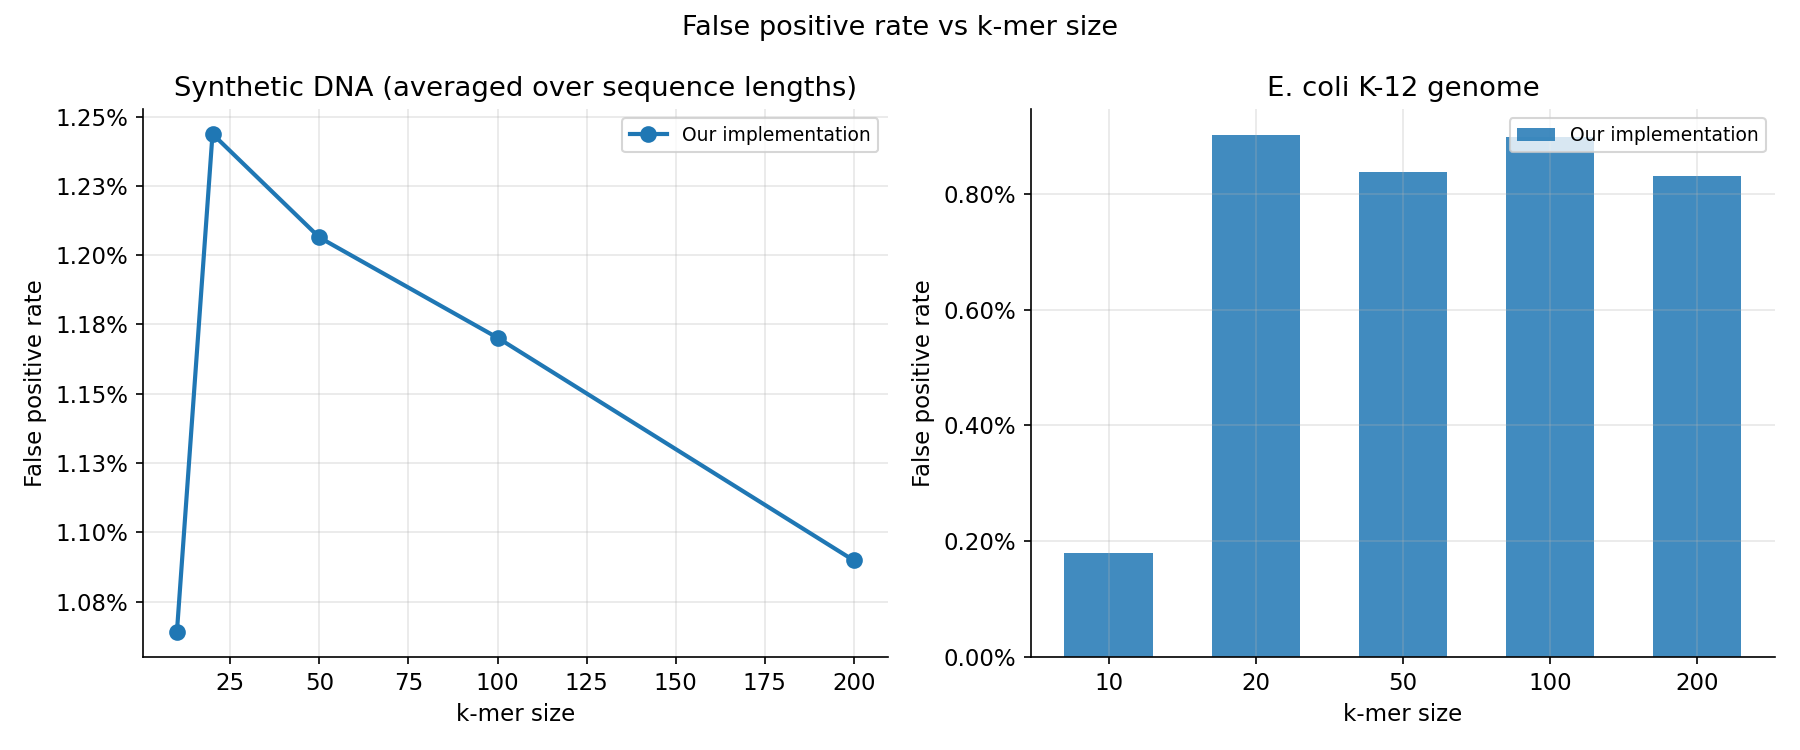
\includegraphics[width=\textwidth]{figures/plot_fpr.png}
    \caption{Lažno-pozitivna stopa u ovisnosti o veličini $k$-mera. Lijevo: sintetički
    podaci, srednja vrijednost preko svih duljina niza. Desno: genom \textit{E.~coli}.
    Niska FPR za $k = 10$ na \textit{E.~coli} posljedica je deduplikacije ponavljanih
    $k$-mera.}
    \label{fig:fpr}
\end{figure}

\subsection{Analiza memorije}
Memorija po elementu (Slika~\ref{fig:memory}) kreće se između 16 i 36 bita za
sintetičke podatke. Teorijski minimum za 12-bitni otisak iznosi $f = 12$ bita;
preostalih 4--24 bita predstavlja:
\begin{itemize}
    \item \textbf{Internu fragmentaciju bucket-a:} svaki bucket alocira 4 utora, ali se
          pri visokoj popunjenosti popuni samo $\sim 90\%$, što dodaje $\sim 10\%$
          overhead-a.
    \item \textbf{Zaokruživanje segmenata na potencije broja 2:} broj segmenata
          udvostručuje se na svakoj razini, pa stvarna alocirana kapacitet može
          biti i dvostruko veći od potrebnog.
\end{itemize}
Na genomu \textit{E.~coli} za $k = 10$ izmjereno je samo 7{,}2 bita po elementu, što
je \emph{ispod} teorijskog minimuma za otisak --- razlog je već spomenuta
deduplikacija: \texttt{num\_inserted} broji \emph{sve} pozive \texttt{Insert} (uključujući
duplikate koji ne zauzimaju nove utore), pa omjer \texttt{memorija/pozivi} izgleda umjetno
nizak. Stvarni broj jedinstvenih otisaka u filteru znatno je manji.

\begin{figure}[H]
    \centering
    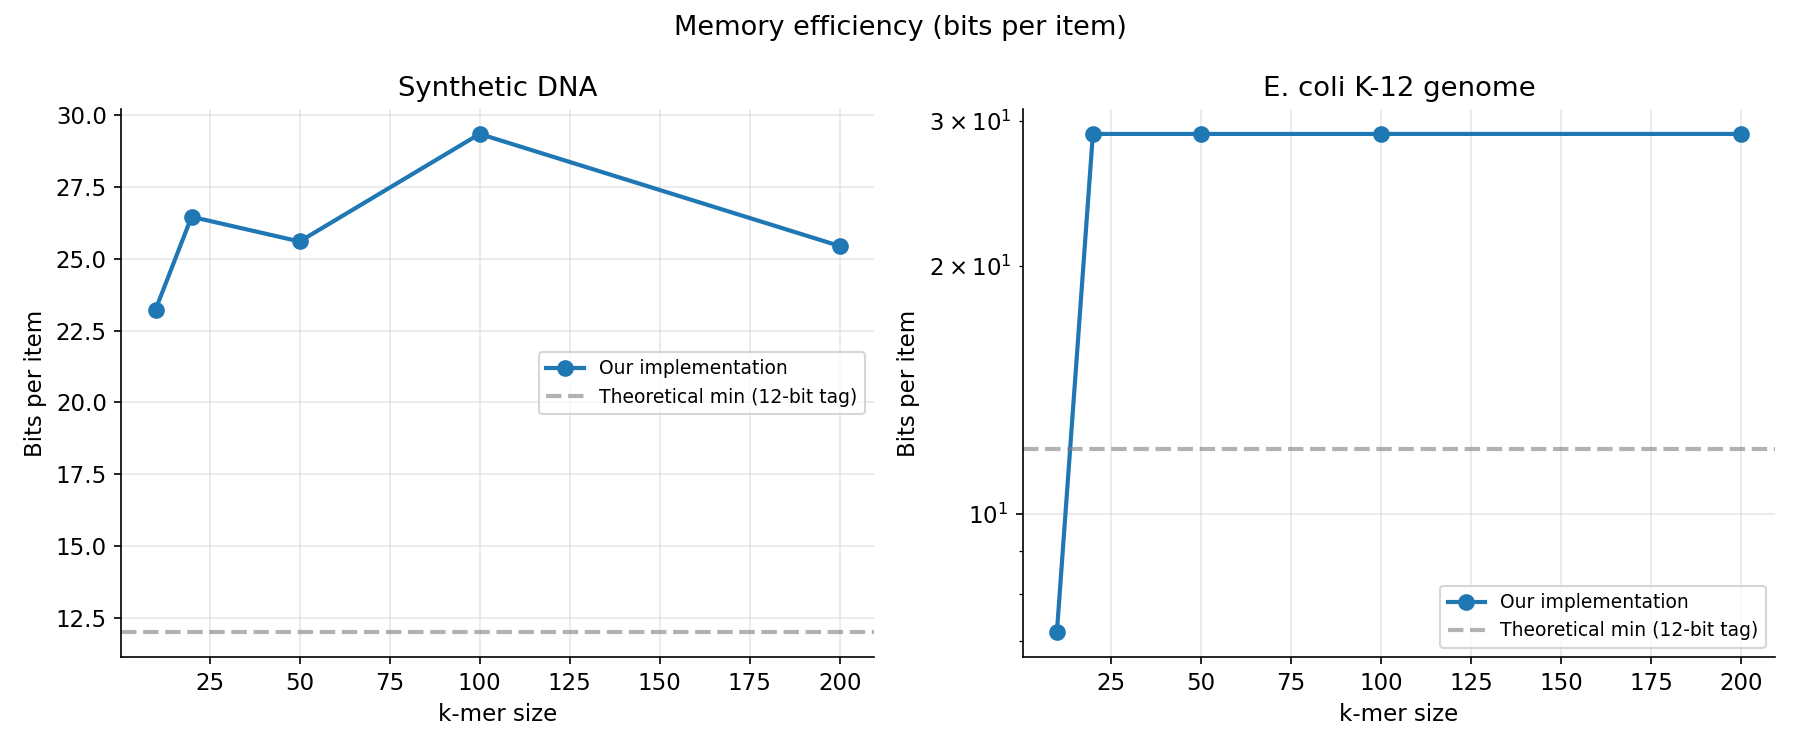
\includegraphics[width=\textwidth]{figures/plot_memory.png}
    \caption{Memorijska efikasnost izražena u bitima po elementu. Iscrtana linija
    označava teorijski minimum od 12 bita (sami otisak). Niža vrijednost za $k = 10$
    na \textit{E.~coli} (desno) posljedica je deduplikacije ponavljanih $k$-mera.}
    \label{fig:memory}
\end{figure}

\subsection{Validacija ispravnosti}
Implementacija je validirana kroz šest jediničnih testova
(\texttt{tests/test\_bamboo.cpp}):
\begin{enumerate}
    \item \textbf{Basic correctness} --- umetanje i pretraživanje tri ručno odabrana
          $k$-mera.
    \item \textbf{Delete} --- ispravnost brisanja, uključujući neuspjeh za nepostojeći
          element.
    \item \textbf{No false negatives} --- nakon umetanja 1000 nasumičnih
          $k$-mera, svi se moraju pronaći (\emph{tvrda garancija} svih Cuckoo-baziranih
          filtera).
    \item \textbf{False positive rate} --- nad 5000 upita FPR mora biti $< 1\%$.
    \item \textbf{Expand} --- nakon dovoljnog broja umetanja broj segmenata se mora
          udvostručiti, a svi prethodno umetnuti $k$-meri i dalje pronaći.
    \item \textbf{Shrink} --- nakon brisanja 75\% elemenata broj segmenata se mora
          smanjiti, a preostali elementi i dalje pronaći.
\end{enumerate}
Svih šest testova prolaze (izlaz \texttt{PASSED} za svaki test).

\subsection{Usporedba s referentnom implementacijom}
\label{sec:reference}
Referentna implementacija autora Wang \textit{et al.}~\cite{wanghanchengchn-repo}
integrirana je u CMake build sustav putem \texttt{FetchContent} mehanizma i dostupna
opcijom \texttt{-DBUILD\_REFERENCE=ON}. Referentni kod koristi AVX2 SIMD intrinzike
(\texttt{\_mm256\_*}) te GCC-specifične proširenja (\texttt{-fpermissive}), te se
stoga može prevoditi samo na Linux/x86\_64 platformi. Naša razvojna platforma (Apple
Silicon ARM64, macOS) ne podržava ova proširenja, te empirijska usporedba nije bila
izvediva u istom okruženju.

\emph{Napomena:} pri demonstraciji projekta na Linux računalu (kako je propisano u
uputama za predaju) referentni benchmark se može pokrenuti naredbom
\texttt{./reference\_benchmark}, a rezultati se zatim združuju s našima pomoću skripte
\texttt{plot.py --mine ... --ref ...} koja generira i graf omjera performansi.

% =====================================================================
% 6. ZAKLJUČAK
% =====================================================================
\section{Zaključak}
\label{sec:zakljucak}

U ovom radu implementirali smo \emph{Bamboo Filter} prema specifikaciji Wang
\textit{et al.}~\cite{wang2022bamboo, wang2024bamboo} u programskom jeziku C++17 i
detaljno ga eksperimentalno procijenili na umjetno generiranim DNK nizovima i na
referentnom genomu \textit{E.~coli} K-12 MG1655. Implementacija ispravno podržava sve
tri ključne operacije (Insert, Lookup, Delete) i obje karakteristične operacije
glatkog dimenzioniranja (Split, Merge), te zadovoljava sve jedinične testove
ispravnosti.

\noindent\textbf{Ključni rezultati:}
\begin{itemize}
    \item Vrijeme umetanja skalira linearno s brojem $k$-mera, što potvrđuje
          amortizirano konstantnu cijenu po umetanju.
    \item FPR pri visokoj popunjenosti iznosi $\sim 1{,}1\%$, oko 5--6$\times$ više od
          teorijskog minimuma od 0{,}2\% --- granica je definirana izabranim pragom
          dijeljenja $\tau_e = 0{,}9$.
    \item Memorijska efikasnost je 21--29 bita po elementu na sintetičkim podacima,
          uz teorijski minimum od 12 bita.
    \item Negativno pretraživanje je 1--2 reda veličine brže od pozitivnog, što je
          očekivano za AMQ filtere s ranim prekidom petlje.
    \item Deduplikacija ponavljanih $k$-mera (problem specifičan za biološke nizove
          kratke $k$) ključna je za stabilnost filtera --- bez nje, duplikati bi doveli
          do beskonačnog dijeljenja.
\end{itemize}

\noindent\textbf{Ograničenja i smjerovi za daljnji rad:}
\begin{itemize}
    \item Empirijska usporedba s referentnom implementacijom autora nije provedena na
          ARM64 platformi; potrebno je pokrenuti na Linux/x86\_64 s AVX2 podrškom.
    \item FPR bi se mogao smanjiti spuštanjem praga dijeljenja $\tau_e$, uz cijenu
          većeg utroška memorije; vrijedi istražiti optimalan kompromis.
    \item Skaliranje na duljine $\geq 10^7$ bp i na druge genome (npr.~kromosom
          čovjeka) bilo bi smisleno proširenje.
    \item Implementacija \emph{semi-sorting} tehnike iz \cite{fan2014cuckoo} dodatno bi
          smanjila utrošak memorije za otprilike 1 bit po elementu.
\end{itemize}

% =====================================================================
% LITERATURA
% =====================================================================
\begin{thebibliography}{99}

\bibitem{wang2022bamboo}
H.~Wang, C.~Yang, B.~Lv, Y.~Gu, J.~Li, S.~Chen i T.~Yang.
\textit{Bamboo Filters: Make Resizing Smooth}.
U: \textit{Proc.~IEEE Int.~Conf.~on Data Engineering (ICDE)}, 2022.
DOI: \href{https://doi.org/10.1109/ICDE53745.2022.00078}{10.1109/ICDE53745.2022.00078}.

\bibitem{wang2024bamboo}
H.~Wang \textit{et al.}
\textit{Bamboo Filters: Make Resizing Smooth and Adaptive}.
\textit{IEEE/ACM Transactions on Networking}, 2024.
DOI: \href{https://doi.org/10.1109/TNET.2024.3403997}{10.1109/TNET.2024.3403997}.

\bibitem{fan2014cuckoo}
B.~Fan, D.~G.~Andersen, M.~Kaminsky i M.~D.~Mitzenmacher.
\textit{Cuckoo Filter: Practically Better Than Bloom}.
U: \textit{Proc.~10th ACM Int.~Conf.~on Emerging Networking Experiments and
Technologies (CoNEXT)}, 2014, str.~75--88.
DOI: \href{https://doi.org/10.1145/2674005.2674994}{10.1145/2674005.2674994}.

\bibitem{fan2013cuckoo}
B.~Fan, D.~G.~Andersen i M.~Kaminsky.
\textit{Cuckoo Filter: Better Than Bloom}.
USENIX \textit{;login:}, vol.~39, no.~4, 2013.
URL: \url{https://www.cs.cmu.edu/~binfan/papers/login_cuckoofilter.pdf}.

\bibitem{bloom1970}
B.~H.~Bloom.
\textit{Space/time trade-offs in hash coding with allowable errors}.
\textit{Communications of the ACM}, vol.~13, no.~7, 1970, str.~422--426.
DOI: \href{https://doi.org/10.1145/362686.362692}{10.1145/362686.362692}.

\bibitem{chen2017dynamic}
H.~Chen, L.~Liao, H.~Jin i J.~Wu.
\textit{The dynamic cuckoo filter}.
U: \textit{Proc.~IEEE 25th Int.~Conf.~on Network Protocols (ICNP)}, 2017.

\bibitem{zhang2021ldcf}
F.~Zhang \textit{et al.}
\textit{The Logarithmic Dynamic Cuckoo Filter}.
U: \textit{Proc.~IEEE Int.~Conf.~on Data Engineering (ICDE)}, 2021.
DOI: \href{https://doi.org/10.1109/ICDE51399.2021.00087}{10.1109/ICDE51399.2021.00087}.

\bibitem{appleby-murmurhash}
A.~Appleby.
\textit{MurmurHash3}, public domain.
URL: \url{https://github.com/aappleby/smhasher}.

\bibitem{ncbi-ecoli}
National Center for Biotechnology Information.
\textit{Escherichia coli str.~K-12 substr.~MG1655, complete genome.}
NCBI Assembly GCA\_000005845.2 (ASM584v2).
URL: \url{https://www.ncbi.nlm.nih.gov/datasets/genome/GCA_000005845.2/}.

\bibitem{wanghanchengchn-repo}
H.~Wang.
\textit{Bamboofilters reference implementation}, GitHub repozitorij.
URL: \url{https://github.com/wanghanchengchn/bamboofilters}.

\bibitem{ferbio1}
Fakultet elektrotehnike i računarstva, Sveučilište u Zagrebu.
\textit{Bioinformatika 1 --- web stranica predmeta}, 2025./2026.
URL: \url{https://www.fer.unizg.hr/predmet/bio1}.

\end{thebibliography}

\end{document}
